\documentclass[tikz,border=4pt,10pt]{standalone}
\usepackage[T1]{fontenc}
\usepackage{lmodern}
\usepackage[scaled=0.92]{helvet}
\renewcommand{\familydefault}{\sfdefault}
\usetikzlibrary{positioning,arrows.meta,calc,fit,backgrounds}

\definecolor{stagefill}{gray}{0.94}
\definecolor{cardfill}{RGB}{255,251,236}
\definecolor{svcfill}{RGB}{234,242,250}
\definecolor{llm}{RGB}{160,60,15}
\definecolor{svc}{RGB}{20,75,145}

\newcommand{\tl}[1]{\textbf{\footnotesize #1}\par\smallskip}
\newcommand{\call}[2]{{\color{llm}\texttt{#1}}\,$\to$\,\texttt{#2}}
\newcommand{\f}[1]{\texttt{#1}}
% A shared service the step uses (legend in the bottom band).
\newcommand{\use}[1]{\tikz[baseline=(t.base)]\node[draw=svc, text=svc, fill=white, rounded corners=1pt,
  inner sep=0.8pt, font=\tiny\bfseries] (t) {#1};}

\tikzset{
  base/.style={draw, align=left, inner sep=3.4pt, font=\scriptsize, anchor=north west},
  stage/.style={base, fill=stagefill, rounded corners=1.5pt, text width=#1},
  part/.style={stage=#1, dashed},
  card/.style={base, fill=cardfill, text width=#1},
  svcbox/.style={base, fill=svcfill, rounded corners=1.5pt, text width=#1},
  flow/.style={-{Stealth[length=2.2mm]}, line width=0.7pt},
}

% Place the next row below the lowest of the given nodes.
\newcommand{\rowbelow}[3]{% name, node a, node b
  \path let \p1=(#2.south), \p2=(#3.south) in coordinate (#1) at (0,{min(\y1,\y2)-0.55cm});}

\begin{document}
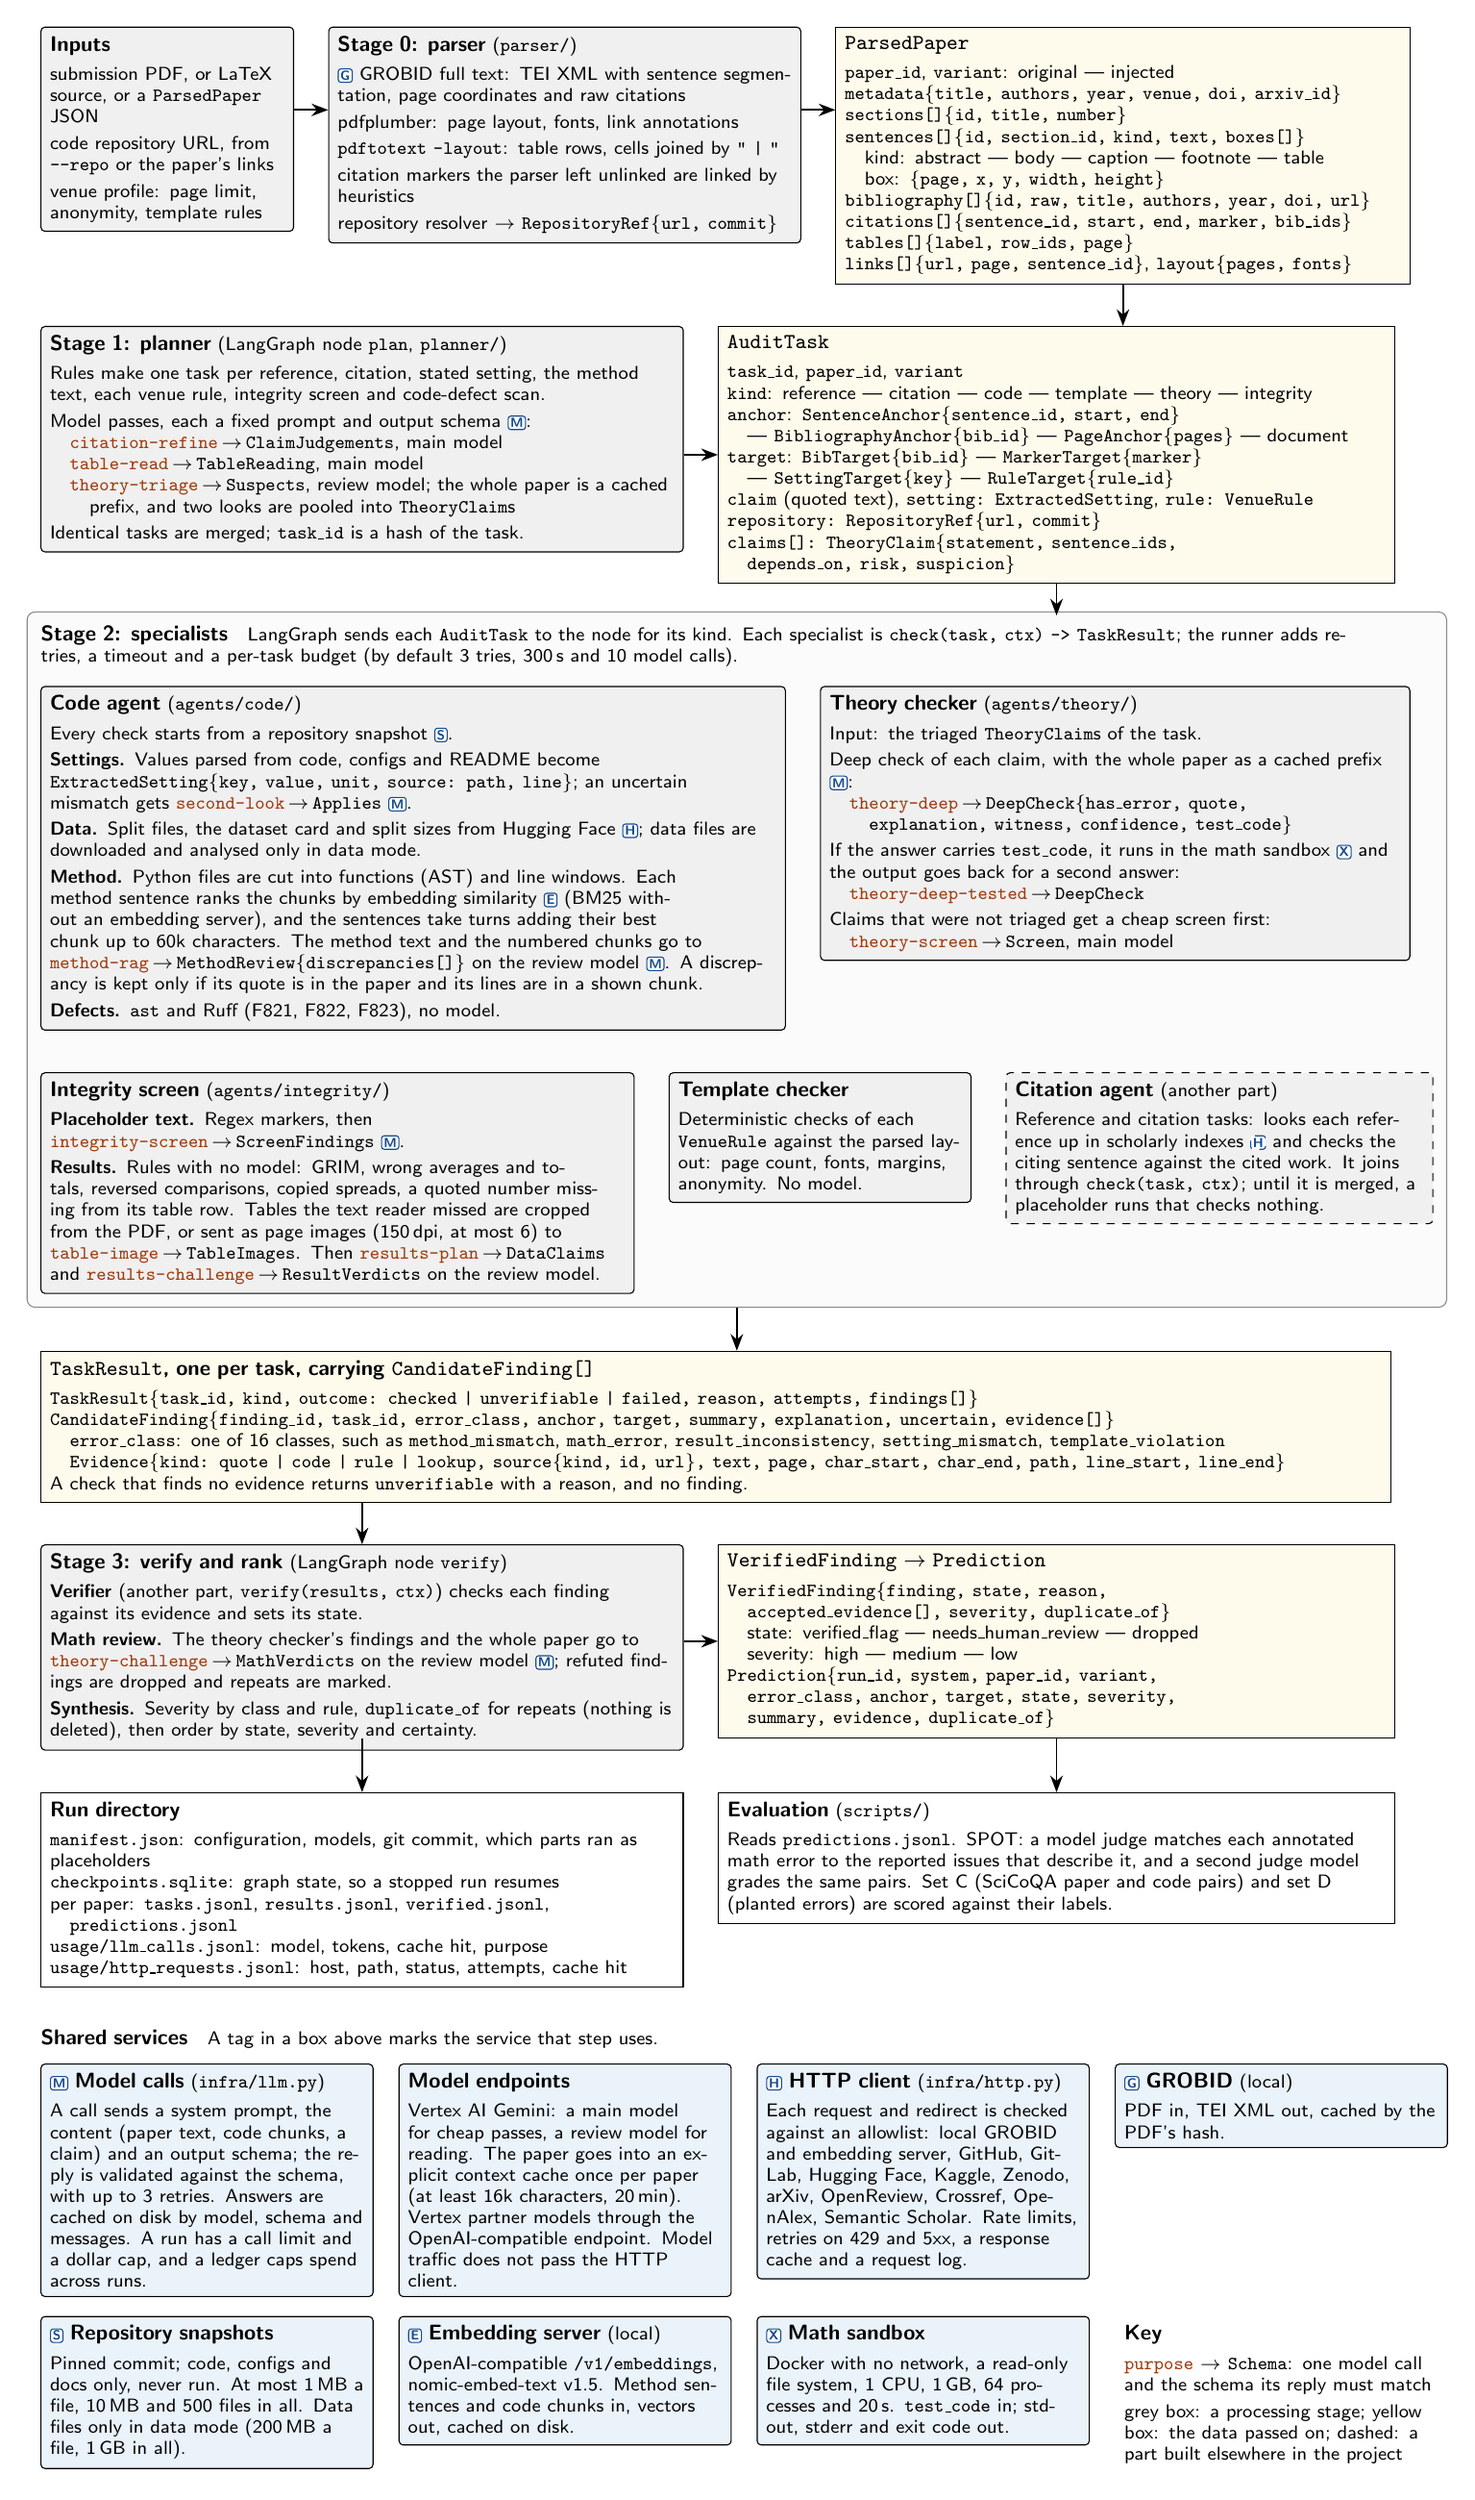
\begin{tikzpicture}

% ================================================================ row 1: inputs, parser, ParsedPaper
\node[stage=3.1cm] (in) at (0,0) {\tl{Inputs}
  submission PDF, or LaTeX source, or a \f{ParsedPaper} JSON\\[2pt]
  code repository URL, from \f{--repo} or the paper's links\\[2pt]
  venue profile: page limit, anonymity, template rules};

\node[stage=6.0cm, right=0.45cm of in.north east, anchor=north west] (parse)
  {\tl{Stage 0: parser \normalfont\scriptsize(\f{parser/})}
  \use{G} GROBID full text: TEI XML with sentence segmentation, page coordinates and raw
  citations\\[2pt]
  pdfplumber: page layout, fonts, link annotations\\[2pt]
  \f{pdftotext -layout}: table rows, cells joined by \f{" | "}\\[2pt]
  citation markers the parser left unlinked are linked by heuristics\\[2pt]
  repository resolver $\to$ \f{RepositoryRef\{url, commit\}}};

\node[card=7.35cm, right=0.45cm of parse.north east, anchor=north west] (pp)
  {\tl{\f{ParsedPaper}}
  \f{paper\_id}, \f{variant}: original | injected\\
  \f{metadata\{title, authors, year, venue, doi, arxiv\_id\}}\\
  \f{sections[]\{id, title, number\}}\\
  \f{sentences[]\{id, section\_id, kind, text, boxes[]\}}\\
  \quad kind: abstract | body | caption | footnote | table\\
  \quad box: \f{\{page, x, y, width, height\}}\\
  \f{bibliography[]\{id, raw, title, authors, year, doi, url\}}\\
  \f{citations[]\{sentence\_id, start, end, marker, bib\_ids\}}\\
  \f{tables[]\{label, row\_ids, page\}}\\
  \f{links[]\{url, page, sentence\_id\}}, \f{layout\{pages, fonts\}}};

\draw[flow] (in.east |- 0,-1.1) -- (parse.west |- 0,-1.1);
\draw[flow] (parse.east |- 0,-1.1) -- (pp.west |- 0,-1.1);

% ================================================================ row 2: planner, AuditTask
\rowbelow{r2}{parse}{pp}
\node[stage=8.25cm] (plan) at (r2) {\tl{Stage 1: planner \normalfont\scriptsize(LangGraph node \f{plan}, \f{planner/})}
  Rules make one task per reference, citation, stated setting, the method text, each venue rule,
  integrity screen and code-defect scan.\\[2pt]
  Model passes, each a fixed prompt and output schema \use{M}:\\
  \quad\call{citation-refine}{ClaimJudgements}, main model\\
  \quad\call{table-read}{TableReading}, main model\\
  \quad\call{theory-triage}{Suspects}, review model; the whole paper is a cached\\
  \qquad prefix, and two looks are pooled into \f{TheoryClaim}s\\[2pt]
  Identical tasks are merged; \f{task\_id} is a hash of the task.};

\node[card=8.7cm, right=0.45cm of plan.north east, anchor=north west] (task)
  {\tl{\f{AuditTask}}
  \f{task\_id}, \f{paper\_id}, \f{variant}\\
  \f{kind}: reference | citation | code | template | theory | integrity\\
  \f{anchor}: \f{SentenceAnchor\{sentence\_id, start, end\}}\\
  \quad | \f{BibliographyAnchor\{bib\_id\}} | \f{PageAnchor\{pages\}} | document\\
  \f{target}: \f{BibTarget\{bib\_id\}} | \f{MarkerTarget\{marker\}}\\
  \quad | \f{SettingTarget\{key\}} | \f{RuleTarget\{rule\_id\}}\\
  \f{claim} (quoted text), \f{setting: ExtractedSetting}, \f{rule: VenueRule}\\
  \f{repository: RepositoryRef\{url, commit\}}\\
  \f{claims[]: TheoryClaim\{statement, sentence\_ids,}\\
  \quad\f{depends\_on, risk, suspicion\}}};

\draw[flow] (pp.south) -- (pp.south |- task.north);
\draw[flow] (plan.east |- task.west) -- (task.west);

% ================================================================ row 3: specialists
\rowbelow{r3}{plan}{task}
\node[base, draw=none, text width=17.6cm, inner sep=0pt] (fan) at (r3)
  {\textbf{\footnotesize Stage 2: specialists}\quad LangGraph sends each \f{AuditTask} to the node
  for its kind. Each specialist is \f{check(task, ctx) -> TaskResult}; the runner adds retries, a
  timeout and a per-task budget (by default 3 tries, 300\,s and 10 model calls).};
\draw[flow] (task.south) -- ++(0,-0.42);

\node[stage=9.6cm, below=0.25cm of fan.south west, anchor=north west] (code)
  {\tl{Code agent \normalfont\scriptsize(\f{agents/code/})}
  Every check starts from a repository snapshot \use{S}.\\[2pt]
  \textbf{Settings.} Values parsed from code, configs and README become
  \f{ExtractedSetting\{key, value, unit, source: path, line\}}; an uncertain mismatch gets
  \call{second-look}{Applies} \use{M}.\\[2pt]
  \textbf{Data.} Split files, the dataset card and split sizes from Hugging Face \use{H}; data
  files are downloaded and analysed only in data mode.\\[2pt]
  \textbf{Method.} Python files are cut into functions (AST) and line windows. Each method
  sentence ranks the chunks by embedding similarity \use{E} (BM25 without an embedding
  server), and the sentences take turns adding their best chunk up to 60k characters. The
  method text and the numbered chunks go to \call{method-rag}{MethodReview\{discrepancies[]\}}
  on the review model \use{M}. A discrepancy is kept only if its quote is in the paper and its
  lines are in a shown chunk.\\[2pt]
  \textbf{Defects.} \f{ast} and Ruff (F821, F822, F823), no model.};

\node[stage=7.55cm, right=0.45cm of code.north east, anchor=north west] (theory)
  {\tl{Theory checker \normalfont\scriptsize(\f{agents/theory/})}
  Input: the triaged \f{TheoryClaim}s of the task.\\[2pt]
  Deep check of each claim, with the whole paper as a cached prefix \use{M}:\\
  \quad\call{theory-deep}{DeepCheck\{has\_error, quote,}\\ \qquad\f{explanation, witness, confidence, test\_code\}}\\[2pt]
  If the answer carries \f{test\_code}, it runs in the math sandbox \use{X} and the output goes
  back for a second answer:\\
  \quad\call{theory-deep-tested}{DeepCheck}\\[2pt]
  Claims that were not triaged get a cheap screen first:\\
  \quad\call{theory-screen}{Screen}, main model};

\rowbelow{r3b}{code}{theory}
\node[stage=7.6cm] (integ) at (r3b) {\tl{Integrity screen \normalfont\scriptsize(\f{agents/integrity/})}
  \textbf{Placeholder text.} Regex markers, then \call{integrity-screen}{ScreenFindings} \use{M}.\\[2pt]
  \textbf{Results.} Rules with no model: GRIM, wrong averages and totals, reversed comparisons,
  copied spreads, a quoted number missing from its table row. Tables the text reader missed
  are cropped from the PDF, or sent as page images (150\,dpi, at most 6) to
  \call{table-image}{TableImages}. Then \call{results-plan}{DataClaims} and
  \call{results-challenge}{ResultVerdicts} on the review model.};

\node[stage=3.75cm, right=0.45cm of integ.north east, anchor=north west] (tmpl)
  {\tl{Template checker}
  Deterministic checks of each \f{VenueRule} against the parsed layout: page count, fonts,
  margins, anonymity. No model.};

\node[part=5.4cm, right=0.45cm of tmpl.north east, anchor=north west] (cite)
  {\tl{Citation agent \normalfont\scriptsize(another part)}
  Reference and citation tasks: looks each reference up in scholarly indexes \use{H} and checks
  the citing sentence against the cited work. It joins through \f{check(task, ctx)}; until it
  is merged, a placeholder runs that checks nothing.};

% ================================================================ row 4: TaskResult
\rowbelow{r4}{integ}{cite}
\path (r4) ++(0,-0.2) coordinate (r4);
\node[card=17.6cm] (res) at (r4) {\tl{\f{TaskResult}, one per task, carrying \f{CandidateFinding[]}}
  \f{TaskResult\{task\_id, kind, outcome: checked | unverifiable | failed, reason, attempts, findings[]\}}\\
  \f{CandidateFinding\{finding\_id, task\_id, error\_class, anchor, target, summary, explanation, uncertain, evidence[]\}}\\
  \quad\f{error\_class}: one of 16 classes, such as \f{method\_mismatch}, \f{math\_error}, \f{result\_inconsistency},
  \f{setting\_mismatch}, \f{template\_violation}\\
  \quad\f{Evidence\{kind: quote | code | rule | lookup, source\{kind, id, url\}, text, page, char\_start, char\_end, path,
  line\_start, line\_end\}}\\
  A check that finds no evidence returns \f{unverifiable} with a reason, and no finding.};

\begin{scope}[on background layer]
  \node[draw=black!45, rounded corners=3pt, fill=black!1.5, inner sep=5pt,
        fit=(fan) (code) (theory) (integ) (tmpl) (cite)] (spec) {};
\end{scope}
\draw[flow] (spec.south) -- (spec.south |- res.north);

% ================================================================ row 5: verify, VerifiedFinding
\node[stage=8.25cm, below=0.55cm of res.south west, anchor=north west] (ver)
  {\tl{Stage 3: verify and rank \normalfont\scriptsize(LangGraph node \f{verify})}
  \textbf{Verifier} (another part, \f{verify(results, ctx)}) checks each finding against its evidence and sets its state.\\[2pt]
  \textbf{Math review.} The theory checker's findings and the whole paper go to
  \call{theory-challenge}{MathVerdicts} on the review model \use{M}; refuted findings are
  dropped and repeats are marked.\\[2pt]
  \textbf{Synthesis.} Severity by class and rule, \f{duplicate\_of} for repeats (nothing is
  deleted), then order by state, severity and certainty.};

\node[card=8.7cm, right=0.45cm of ver.north east, anchor=north west] (vf)
  {\tl{\f{VerifiedFinding} $\to$ \f{Prediction}}
  \f{VerifiedFinding\{finding, state, reason,}\\
  \quad\f{accepted\_evidence[], severity, duplicate\_of\}}\\
  \quad state: verified\_flag | needs\_human\_review | dropped\\
  \quad severity: high | medium | low\\
  \f{Prediction\{run\_id, system, paper\_id, variant,}\\
  \quad\f{error\_class, anchor, target, state, severity,}\\
  \quad\f{summary, evidence, duplicate\_of\}}};

\draw[flow] (res.south -| ver.north) -- (ver.north);
\draw[flow] (ver.east |- vf.west) -- (vf.west);

% ================================================================ row 6: outputs and evaluation
\rowbelow{r6}{ver}{vf}
\node[base, text width=8.25cm] (out) at (r6) {\tl{Run directory}
  \f{manifest.json}: configuration, models, git commit, which parts ran as placeholders\\
  \f{checkpoints.sqlite}: graph state, so a stopped run resumes\\
  per paper: \f{tasks.jsonl}, \f{results.jsonl}, \f{verified.jsonl},\\
  \quad\f{predictions.jsonl}\\
  \f{usage/llm\_calls.jsonl}: model, tokens, cache hit, purpose\\
  \f{usage/http\_requests.jsonl}: host, path, status, attempts, cache hit};

\node[base, text width=8.7cm, right=0.45cm of out.north east, anchor=north west] (eval)
  {\tl{Evaluation \normalfont\scriptsize(\f{scripts/})}
  Reads \f{predictions.jsonl}. SPOT: a model judge matches each annotated math error to the
  reported issues that describe it, and a second judge model grades the same pairs. Set C
  (SciCoQA paper and code pairs) and set D (planted errors) are scored against their labels.};

\draw[flow] (vf.south -| out.north) -- (out.north);
\draw[flow] (vf.south -| eval.north) -- (eval.north);

% ================================================================ row 7: shared services
\rowbelow{r7}{out}{eval}
\node[base, draw=none, inner sep=0pt, text width=17.6cm] (svch) at (r7)
  {\textbf{\footnotesize Shared services}\quad A tag in a box above marks the service that step uses.};

\node[svcbox=4.15cm, below=0.2cm of svch.south west, anchor=north west] (sM)
  {\tl{\use{M} Model calls \normalfont\scriptsize(\f{infra/llm.py})}
  A call sends a system prompt, the content (paper text, code chunks, a claim) and an output
  schema; the reply is validated against the schema, with up to 3 retries. Answers are cached
  on disk by model, schema and messages. A run has a call limit and a dollar cap, and a ledger
  caps spend across runs.};

\node[svcbox=4.15cm, right=0.33cm of sM.north east, anchor=north west] (sV)
  {\tl{Model endpoints}
  Vertex AI Gemini: a main model for cheap passes, a review model for reading. The paper goes
  into an explicit context cache once per paper (at least 16k characters, 20\,min). Vertex
  partner models through the OpenAI-compatible endpoint. Model traffic does not pass the HTTP
  client.};

\node[svcbox=4.15cm, right=0.33cm of sV.north east, anchor=north west] (sH)
  {\tl{\use{H} HTTP client \normalfont\scriptsize(\f{infra/http.py})}
  Each request and redirect is checked against an allowlist: local GROBID and embedding
  server, GitHub, GitLab, Hugging Face, Kaggle, Zenodo, arXiv, OpenReview, Crossref, OpenAlex,
  Semantic Scholar. Rate limits, retries on 429 and 5xx, a response cache and a request log.};

\node[svcbox=4.15cm, right=0.33cm of sH.north east, anchor=north west] (sG)
  {\tl{\use{G} GROBID \normalfont\scriptsize(local)}
  PDF in, TEI XML out, cached by the PDF's hash.};

\node[svcbox=4.15cm, below=0.25cm of sM.south west, anchor=north west] (sS)
  {\tl{\use{S} Repository snapshots}
  Pinned commit; code, configs and docs only, never run. At most 1\,MB a file, 10\,MB and
  500 files in all. Data files only in data mode (200\,MB a file, 1\,GB in all).};

\node[svcbox=4.15cm, right=0.33cm of sS.north east, anchor=north west] (sE)
  {\tl{\use{E} Embedding server \normalfont\scriptsize(local)}
  OpenAI-compatible \f{/v1/embeddings}, nomic-embed-text v1.5. Method sentences and code
  chunks in, vectors out, cached on disk.};

\node[svcbox=4.15cm, right=0.33cm of sE.north east, anchor=north west] (sX)
  {\tl{\use{X} Math sandbox}
  Docker with no network, a read-only file system, 1 CPU, 1\,GB, 64 processes and 20\,s.
  \f{test\_code} in; stdout, stderr and exit code out.};

\node[base, draw=none, text width=4.15cm, right=0.33cm of sX.north east, anchor=north west] (key)
  {\tl{Key}
  {\color{llm}\f{purpose}} $\to$ \f{Schema}: one model call and the schema its reply must
  match\\[2pt]
  grey box: a processing stage; yellow box: the data passed on; dashed: a part built
  elsewhere in the project};

\end{tikzpicture}
\end{document}
